\chapter{改善项目的沟通}
\section{沟通管理概述}
管理沟通把管理学和传播学紧密结合在一起,成为一门跨学科发展的课程体系。
\par 管理学的内容主要包含:管理沟通形态、公共关系沟通、企业沟通、内部沟通技巧、商务沟通。
\subsection{沟通的概念}
沟通相对项目沟通有着更广的外延和更庞大的知识体系,沟通就是意义的传递和理解。这里的意义主要是指信息、思想与情感。 
\par 项目沟通是为实现项目管理目标,项目团队与其他组织、项目团队成员之间信息、思想、情感的传递和理解的过程。 
\par 沟通的作用:
\begin{enumerate}
	\item 沟通是组织内部管理的基础、是协调组织内部关系的纽带,是使组织和项目团队成为一个整体的凝聚剂。
	\item 沟通是领导人或项目经理激励下属,实现领导职能的基本途径。
	\item 沟通是组织或项目团队与外部建立联系的桥梁。
\end{enumerate}
软件项目成功的三个主要因素:用户参与、主管层的支持、需求的清晰表述。
\par 注:对软件项目成功威胁最大的是沟通的失败。
\subsection{沟通的过程}
\begin{figure}[!h]
	\centering
	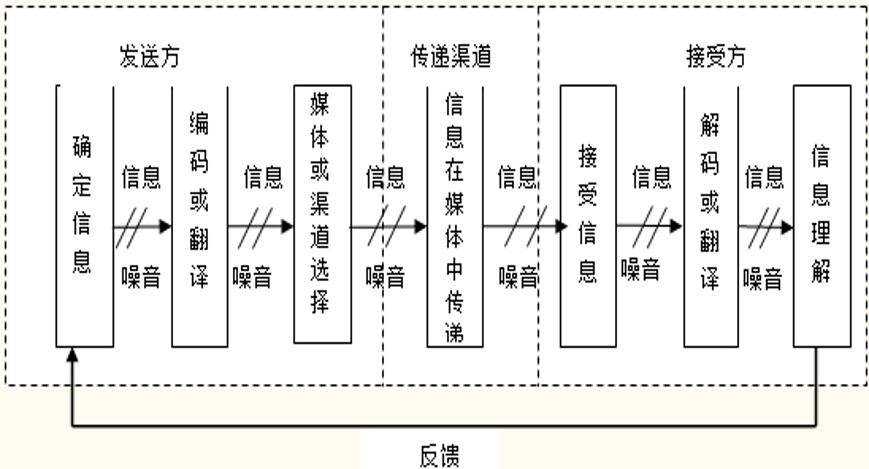
\includegraphics[width=0.8\textwidth]{image/9-1}
	\caption{沟通过程的一般模型}
\end{figure}
\subsection{沟通的类别}
根据不同的分类标准,沟通有如下几种类型:
\begin{itemize}
	\item 按功能划分:工具式沟通与感情式沟通
	\item 按组织系统划分:正式沟通和非正式沟通
	\item 按沟通方向划分:纵向沟通和横向沟通
	\item 按是否进行反馈:单向沟通和双向沟通
	\item 按表达方式、方法:口头沟通和非言语沟通
\end{itemize}
\begin{figure}[!h]
	\centering
	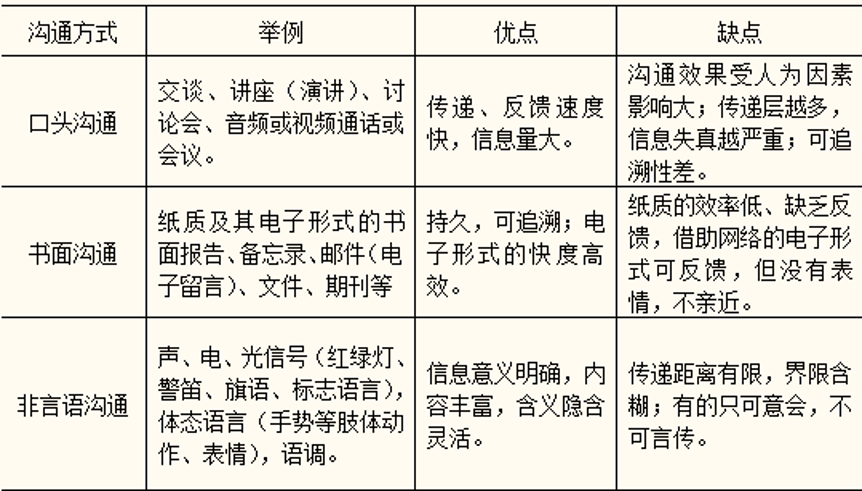
\includegraphics[width=0.8\textwidth]{image/9-2}
	\caption{各种不同表达方式或方法的沟通比较}
\end{figure}
\subsection{沟通网络}
沟通网络是指组织中沟通渠道结构和类型,基本特征有,渠道路径的数量、分布及反馈。几种常见的双向沟通网络模型如图:
\begin{figure}[!h]
	\centering
	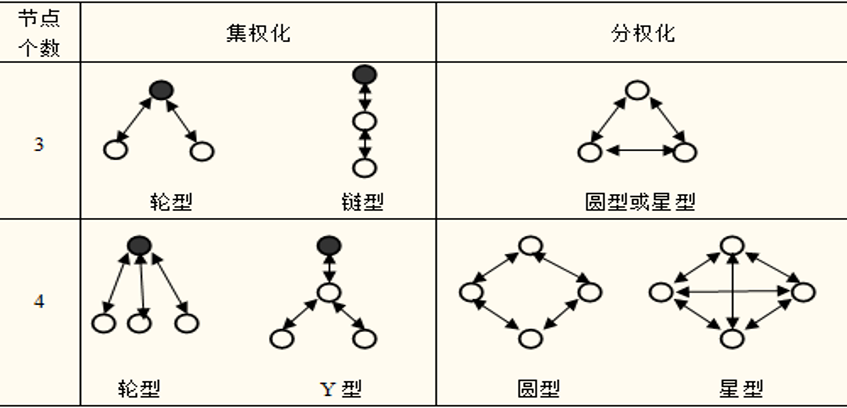
\includegraphics[width=0.8\textwidth]{image/9-3}
	\caption{几种常见的双向沟通网络模型}
\end{figure}
\subsection{项目沟通管理}
项目沟通管理是建立在管理沟通的基础上,服务于项目管理及项目干系人的共同利益。IT项目沟通管理主要过程如图:
\begin{figure}[!h]
	\centering
	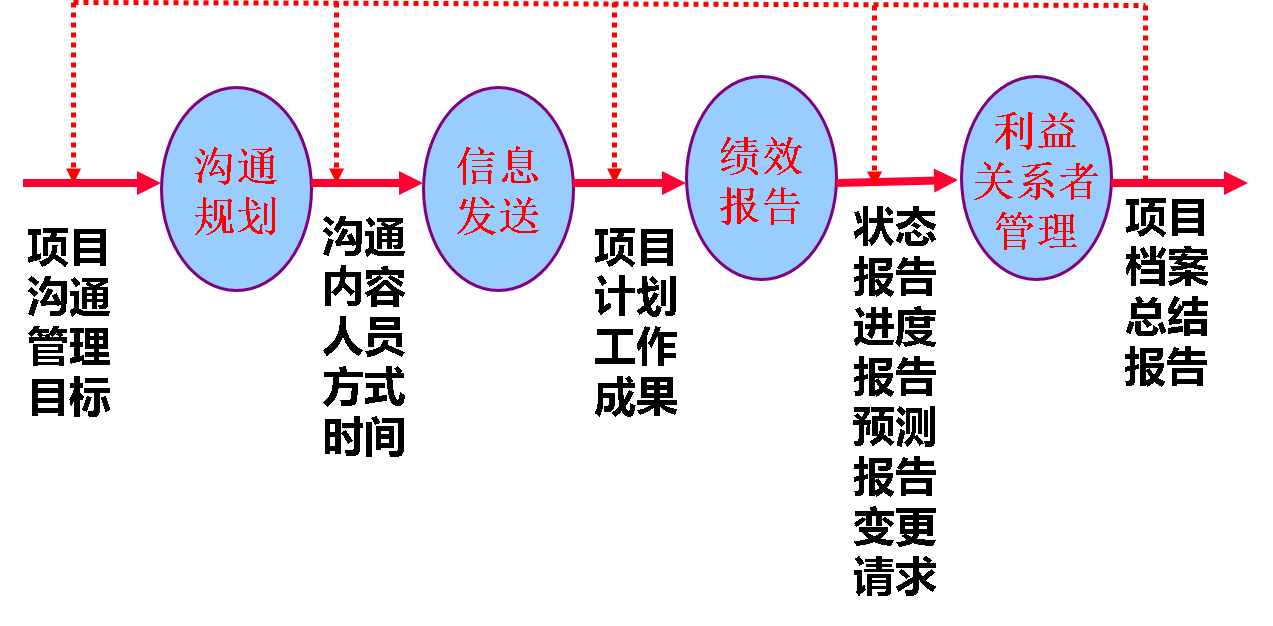
\includegraphics[width=0.8\textwidth]{image/9-4}
	\caption{IT项目沟通管理主要过程}
\end{figure}
\par 项目沟通管理的目标:及时而适当地创建、收集、发送、储存和处理项目的信息。
\section{沟通规划}
沟通规划的核心:了解项目干系人的需求,制定项目沟通管理计划。
\par 规划的主要内容:
\begin{itemize}
	\item 信息收集和存储渠道的结构。
	\item 信息分发渠道的结构。
	\item 分发信息说明。
	\item 进度安排。
	\item 评估信息的方法。
	\item 更新及修订沟通管理计划的方法。
\end{itemize}
\section{信息发布}
信息发布是向项目干系人及时地提供所需的信息,包括实施沟通管理计划以及对预料之外的信息索取要求的应对。
\par 信息收集和检索方式:手工存档系统、电子数据库、项目管理软件以及允许查问诸如工作图纸、设计规范、测试计划持技术文档系统。
\section{绩效报告}
绩效报告的编制需要项目经理和项目组成员对项目的实际执行情况和发展趋势的正确评估和预测。主要工具和技术:
\begin{itemize}
	\item 信息演示工具 
	\item 绩效信息收集和汇总
	\item 状态审查会议 
	\item 工时汇报系统 
	\item 费用汇报系统
\end{itemize}
\section{绩效报告的结果}
绩效报告组织与归纳所收集到的信息,并展示依据绩效衡量基准分析的所有结果。 
\begin{itemize}
	\item 状况报告:描述项目在某一特定时间点所处的项目阶段。状况报告是从达到范围、时间和成本三项目标上分析项目所处的状态。 
	\item 进展报告:描述项目组在某一特定时间工作完成情况。 
	\item 项目预测:预测项目的将来状况与进展。 
	\item 状态评审会议:定期进行的交流有关项目信息的事件。
\end{itemize}
\section{利害关系者管理}
利害关系者(项目干系人)管理,指对沟通进行管理,以满足项目干系人的需求并与他们一起解决问题。
\subsection{遵循沟通原则}
\begin{itemize}
	\item 尽早沟通
	\item 主动沟通
	\item 内外有别
	\item 采用对方能接受的沟通风格 
	\item 沟通的升级原则
\end{itemize}
\subsection{影响项目沟通的因素}
语义上的障碍、知识经验水平的限制、知觉的选择性、心理因素的影响、组织结构的影响、沟通渠道的选择、信息量的多少。
\subsection{使用沟通技巧}
见图9.5和9.6:
\begin{figure}[!h]
	\centering
	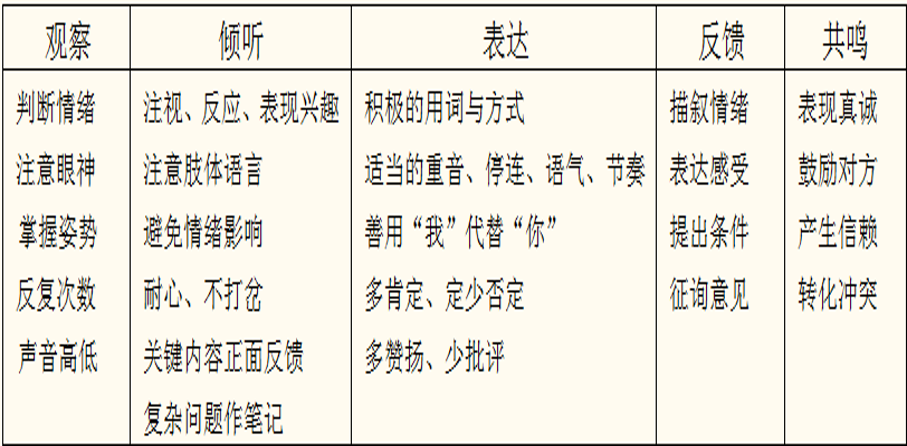
\includegraphics[width=0.8\textwidth]{image/9-5}
	\caption{按沟通过程划分的技巧}
\end{figure}
\begin{figure}[!h]
	\centering
	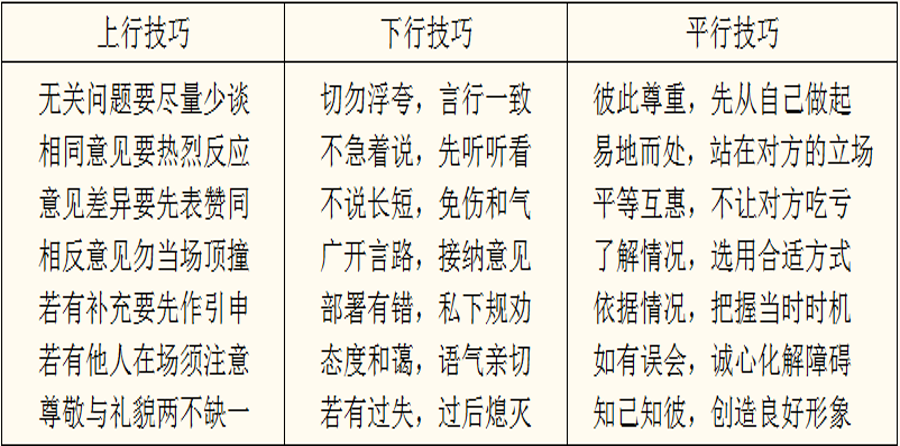
\includegraphics[width=0.8\textwidth]{image/9-6}
	\caption{按不同沟通信息方向划分的技巧}
\end{figure}
\subsection{项目沟通管理工具与模板}
\par 关键词:谈话10大禁忌
\par 项目沟通管理工具与模板见图9.7和9.8:
\begin{figure}[!h]
	\centering
	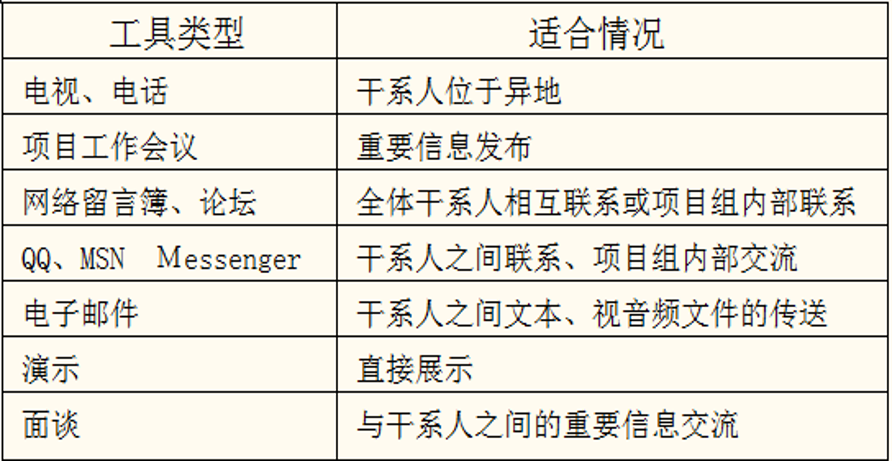
\includegraphics[width=0.8\textwidth]{image/9-7}
	\caption{常用的沟通工具}
\end{figure}
\begin{figure}[!h]
	\centering
	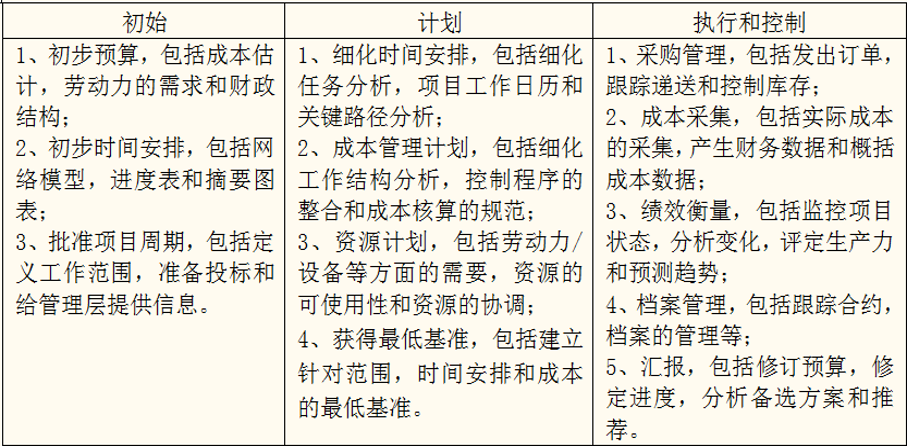
\includegraphics[width=0.8\textwidth]{image/9-8}
	\caption{项目管理软件功能}
\end{figure}
\subsection{良好的冲突管理}
项目冲突是组织冲突的一种特定表现形态,是项目内部或外部某些关系难以协调而导致的矛盾激化和行为对抗。
\subsubsection*{常见的冲突来源}
资源的冲突、费用冲突、技术意见和性能权衡的冲突、管理程序上的冲突、项目优先权的冲突、项目进度的冲突、项目成员个性冲突。
\subsubsection*{项目冲突产生的原因}
沟通与知觉差异、角色混淆、资源分配及利益格局的变化、目标差异。
\subsubsection*{项目冲突的类型}
\begin{itemize}
	\item 建设性冲突或良性冲突
	\item 破坏性冲突 
\end{itemize}
\subsubsection*{解决项目冲突的策略}
回避或撤出、竞争或强制、缓和与调停、妥协 、面对与正视 。